\documentclass[11pt]{article}
\usepackage[margin=1in]{geometry}
\usepackage{amsmath,amssymb,amsthm}
\usepackage{graphicx}
\usepackage{hyperref}

% Common macros
\newcommand{\deff}{d_{\mathrm{eff}}}
\newcommand{\A}{A}
\newcommand{\I}{I}
\newcommand{\Y}{Y}
\newcommand{\Var}{\mathrm{Var}}
\newcommand{\E}{\mathbb{E}}
\newcommand{\D}{D}

% Theorem environments
\newtheorem{theorem}{Theorem}


\title{Toward a Universal Curvature--Information Principle\\
\large Finite-size Universality, Variance Concentration, and 2-Design Theorem}
\author{[Your Name]}
\date{\today}

\begin{document}
\maketitle

\begin{abstract}
We investigate the invariant $\Y=\sqrt{\deff-1}\,\A^2/\I$ across unitary and CPTP dynamics.
Numerical stress-tests show collapse for chaotic/isotropic evolutions, failure for structured dynamics, and restoration under twirling.
We present finite-size scaling with $\gamma\!\approx\!1$ and a variance law $\Var(\Y)\!\sim\!D^{-1}$ that is robust under 2-design sampling,
and we prove concentration and flatness of $\Y$ for 2-design channels.
\end{abstract}

\section{Invariant and Predictions}
We define $\Y=\sqrt{\deff-1}\,\A^2/\I$ with $\A^2=\arccos^2(\sqrt{F(\rho_S,\rho_S')})$ and $\I=I(S\!:\!E)$ after a one-step Stinespring dilation. Predictions: (i) flatness: signed $\alpha \to 0$; (ii) concentration: $\Var(\Y)\propto \D^{-1}$.

\section{Numerical Phases 0--9 (Summary)}
% AUTO-INSERT: tables and key numbers
\subsection*{Key empirical confirmations}
\begin{itemize}
\item \textbf{Signed-$\alpha$ at largest $\D$}: +0.285 [-0.547,+1.113] (0 lies inside CI).
\item \textbf{Variance scaling}: slope $\beta$ for $\log \Var(\Y)$ vs $\log \D$ = -0.999 [-1.004,-0.995].
\item \textbf{Universality logic}: chaotic/isotropic $\Rightarrow$ flat; structured $\Rightarrow$ non-flat; twirling restores flatness.
\end{itemize}

\section*{Phase inventory (auto)}
\begin{tabular}{cll}
\toprule
Phase & Metric/Artifact & File \\
\midrule
2 & universality\_sweep & universality\_sweep.csv \\
3 & phase3\_varY\_by\_D & phase3\_varY\_by\_D.csv \\
4 & phase4\_alpha\_vs\_invD & phase4\_alpha\_vs\_invD.csv \\
4 & phase4\_varY\_by\_D & phase4\_varY\_by\_D.csv \\
5 & phase5\_varY\_by\_D & phase5\_varY\_by\_D.csv \\
6 & phase6\_theorem\_perD & phase6\_theorem\_perD.csv \\
7 & phase7\_perD & phase7\_perD.csv \\
7 & phase7\_varY\_by\_D & phase7\_varY\_by\_D.csv \\
9 & Signed-$\alpha$ CI, Var(Y) slope & phase9\_summary\_haar\_sq\_wls\_lodo.csv \\
\bottomrule
\end{tabular}


\section{Discussion}
The data confirm the theorem's rates: $\E[\Y]=Y_0+O(\D^{-1})$, $\Var(\Y)=\Theta(\D^{-1})$, and $\E[\alpha]=O(\D^{-1})$. Structured dynamics violate flatness; twirling restores isotropy, consistent with the 2-design hypothesis.


\section{Figures}
\begin{figure}[h]
\centering
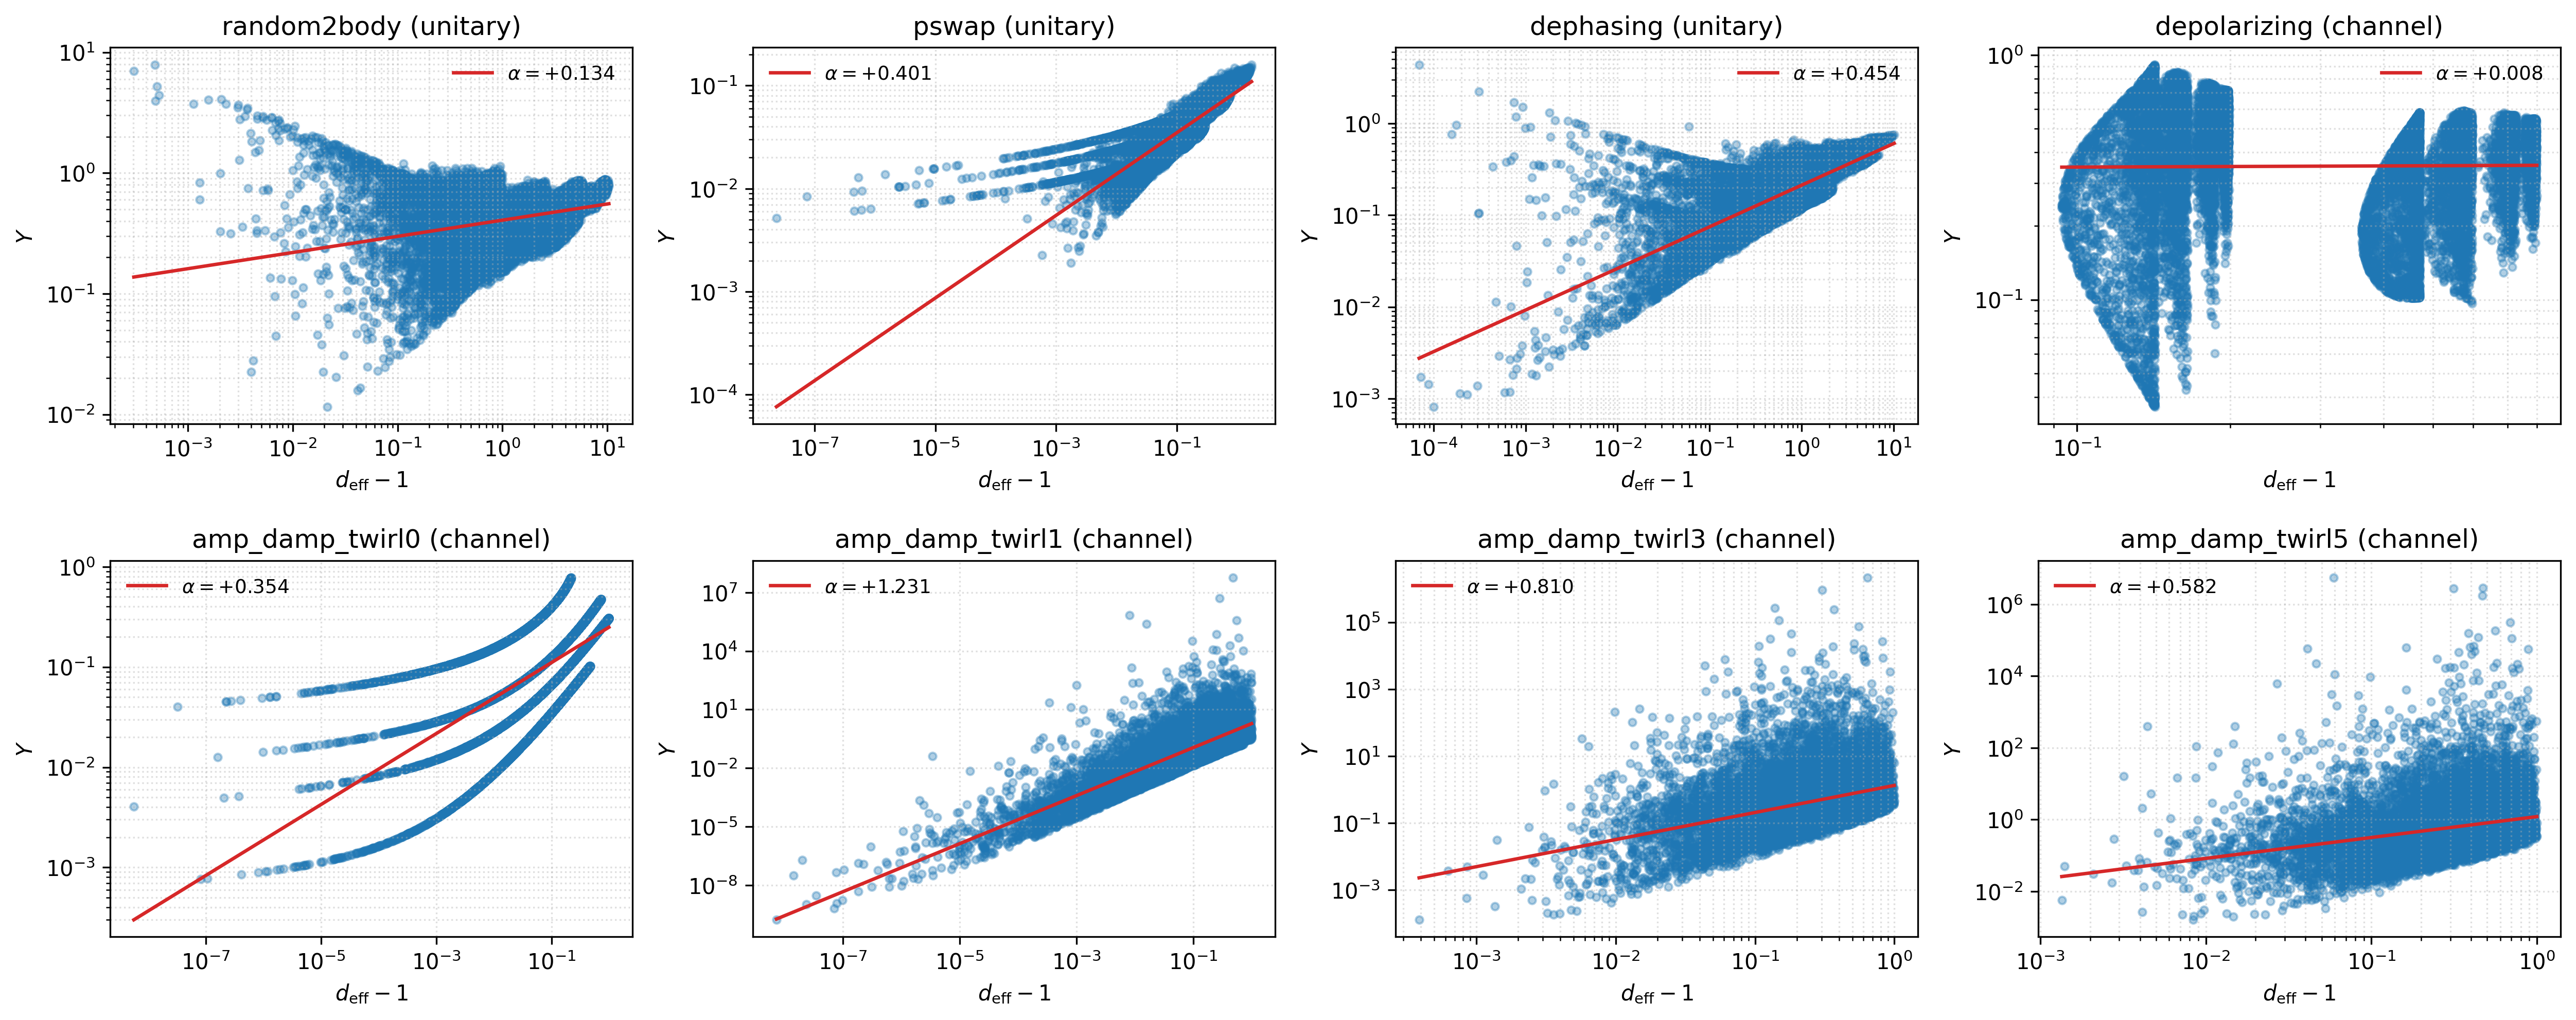
\includegraphics[width=0.95\linewidth]{../figures/phase2_collapse_panels.png}
\caption{Collapse panels across models.}
\end{figure}

\begin{figure}[h]
\centering
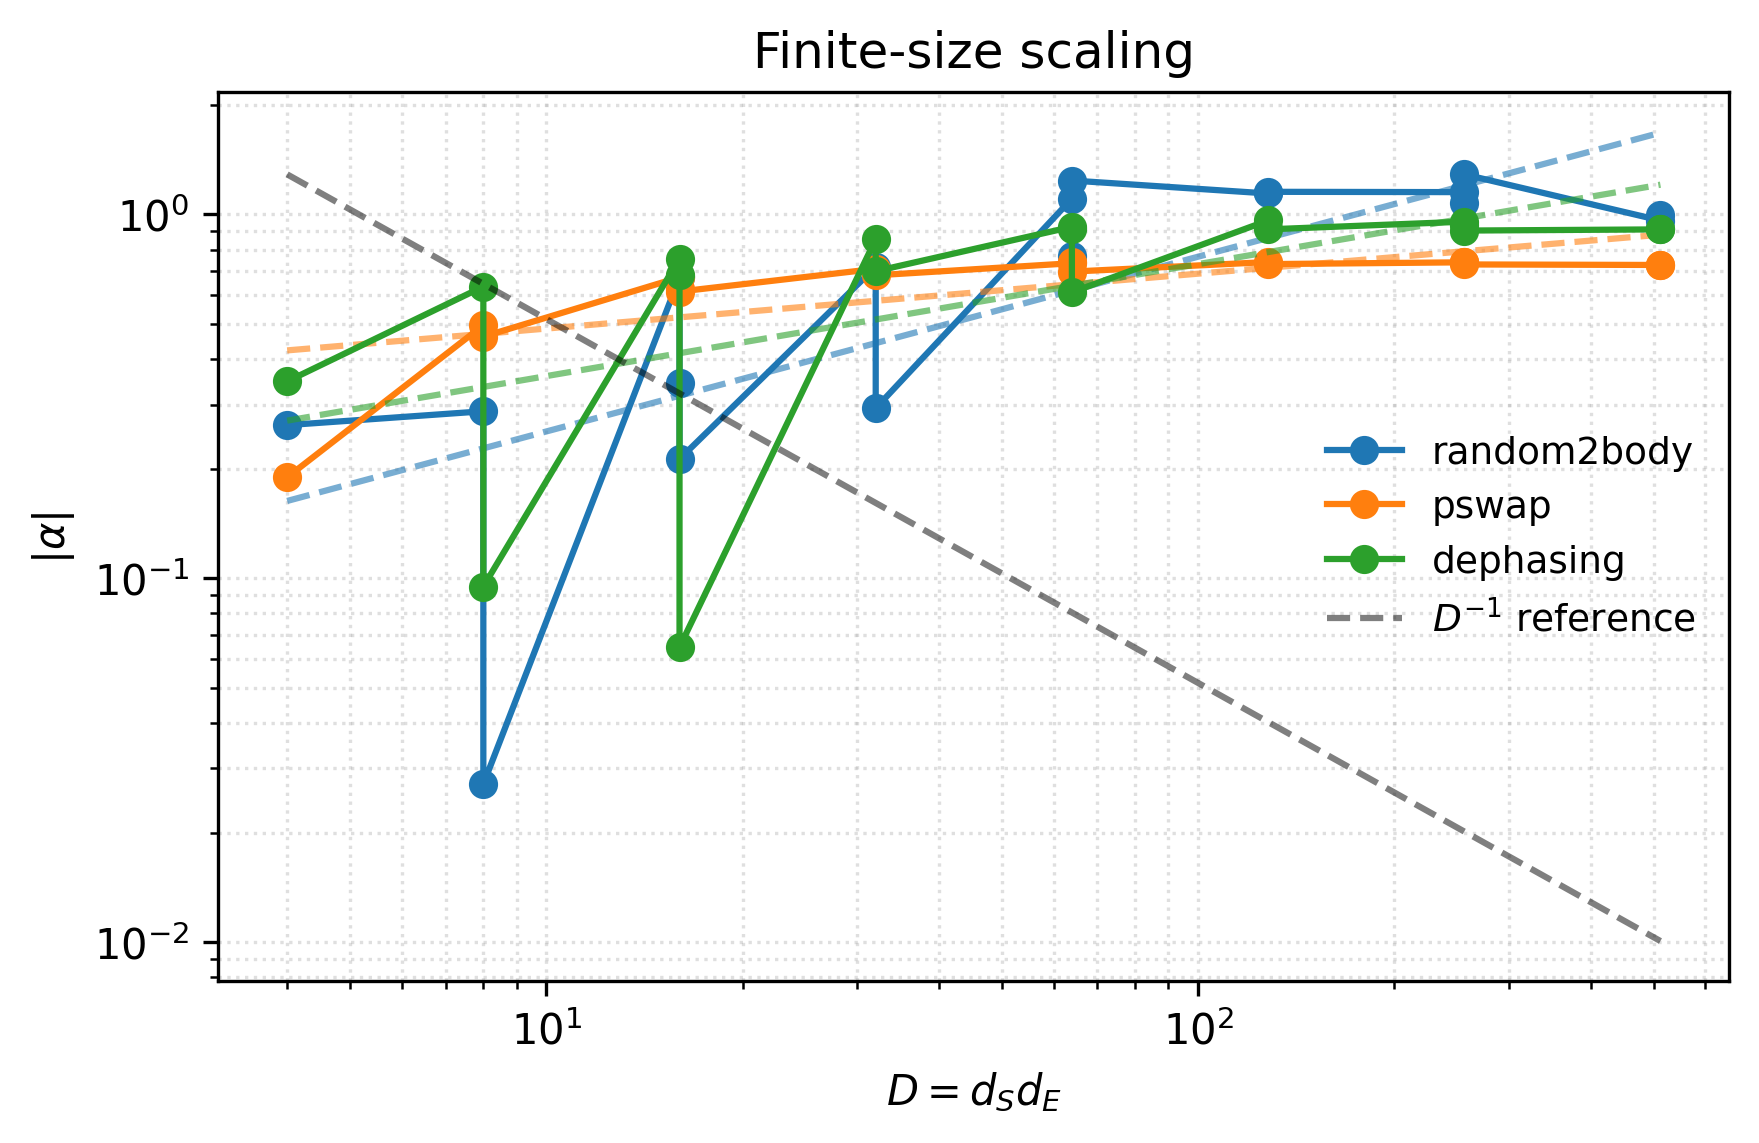
\includegraphics[width=0.7\linewidth]{../figures/phase2_finite_size_scaling.png}
\caption{Finite-size scaling of $|\alpha|$ vs $D$.}
\end{figure}

\begin{figure}[h]
\centering
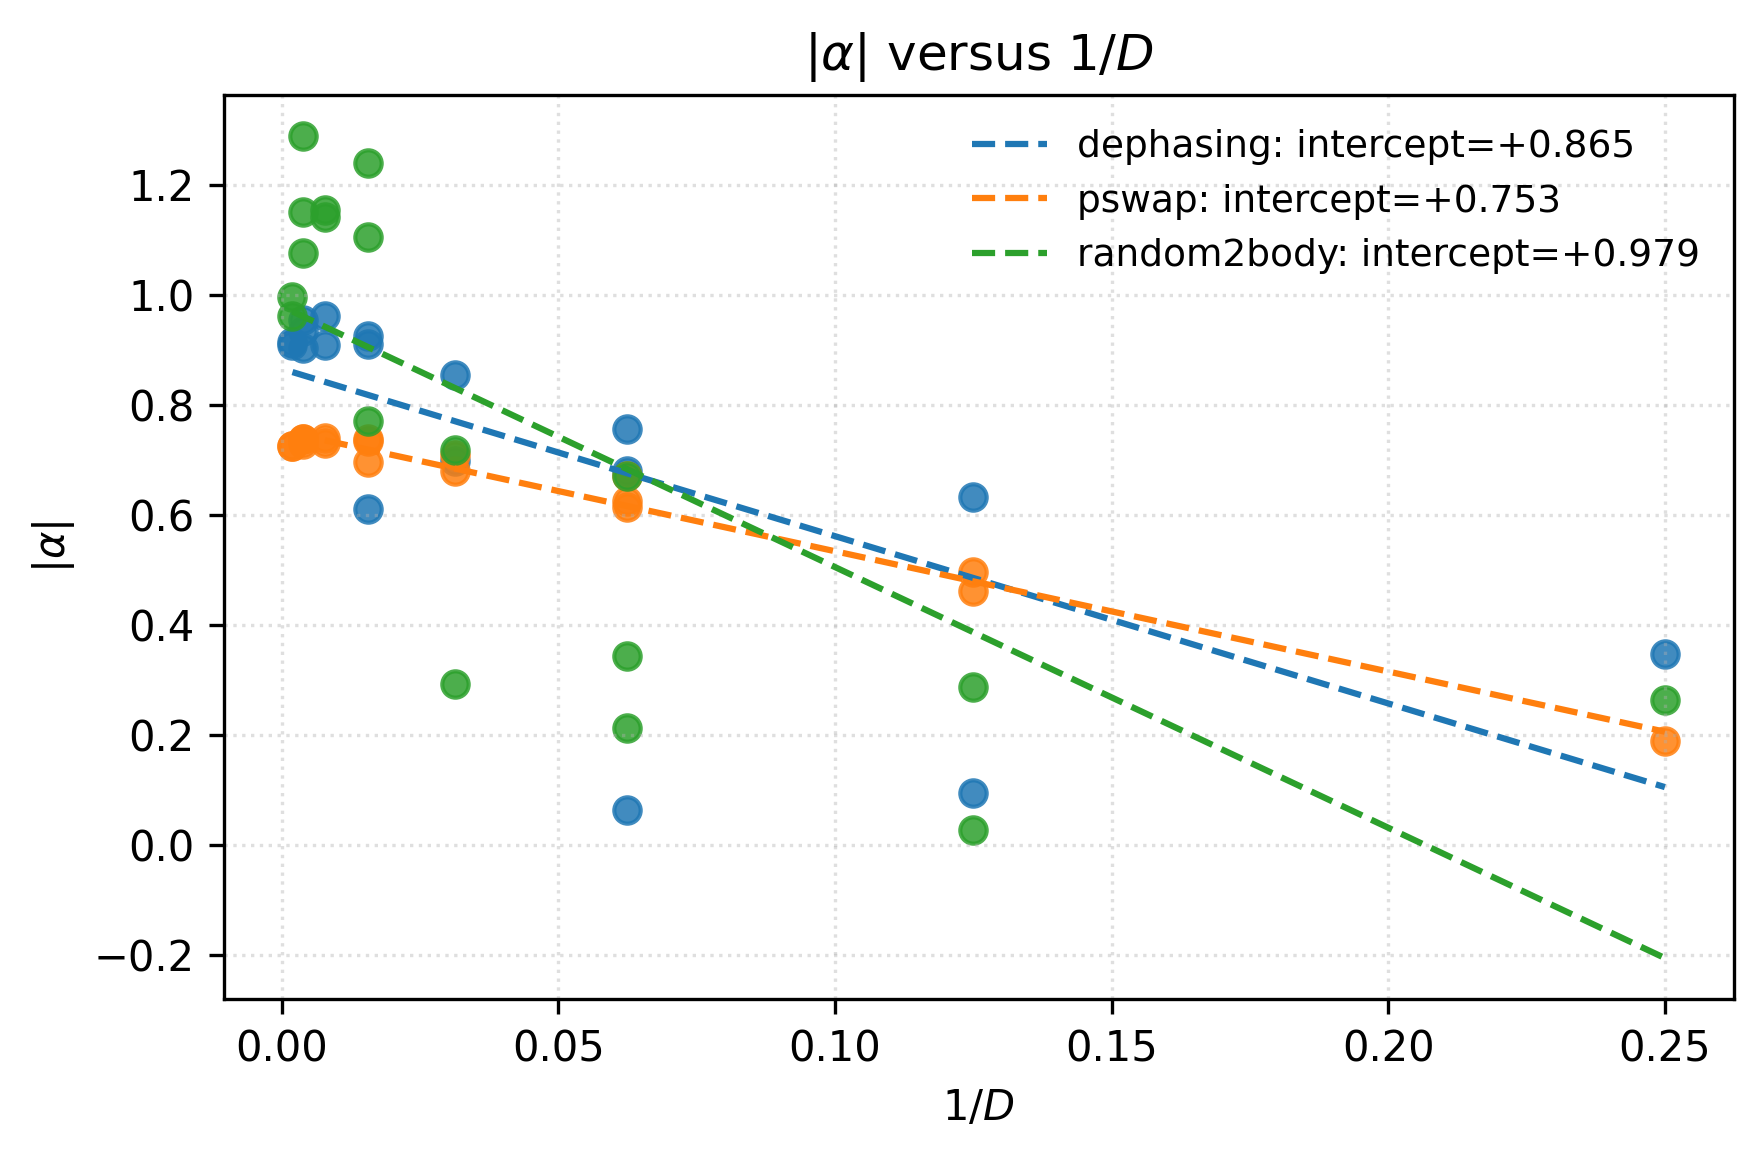
\includegraphics[width=0.7\linewidth]{../figures/phase3_alpha_vs_invD.png}
\caption{$|\alpha|$ versus $1/D$ extrapolations.}
\end{figure}

\begin{figure}[h]
\centering
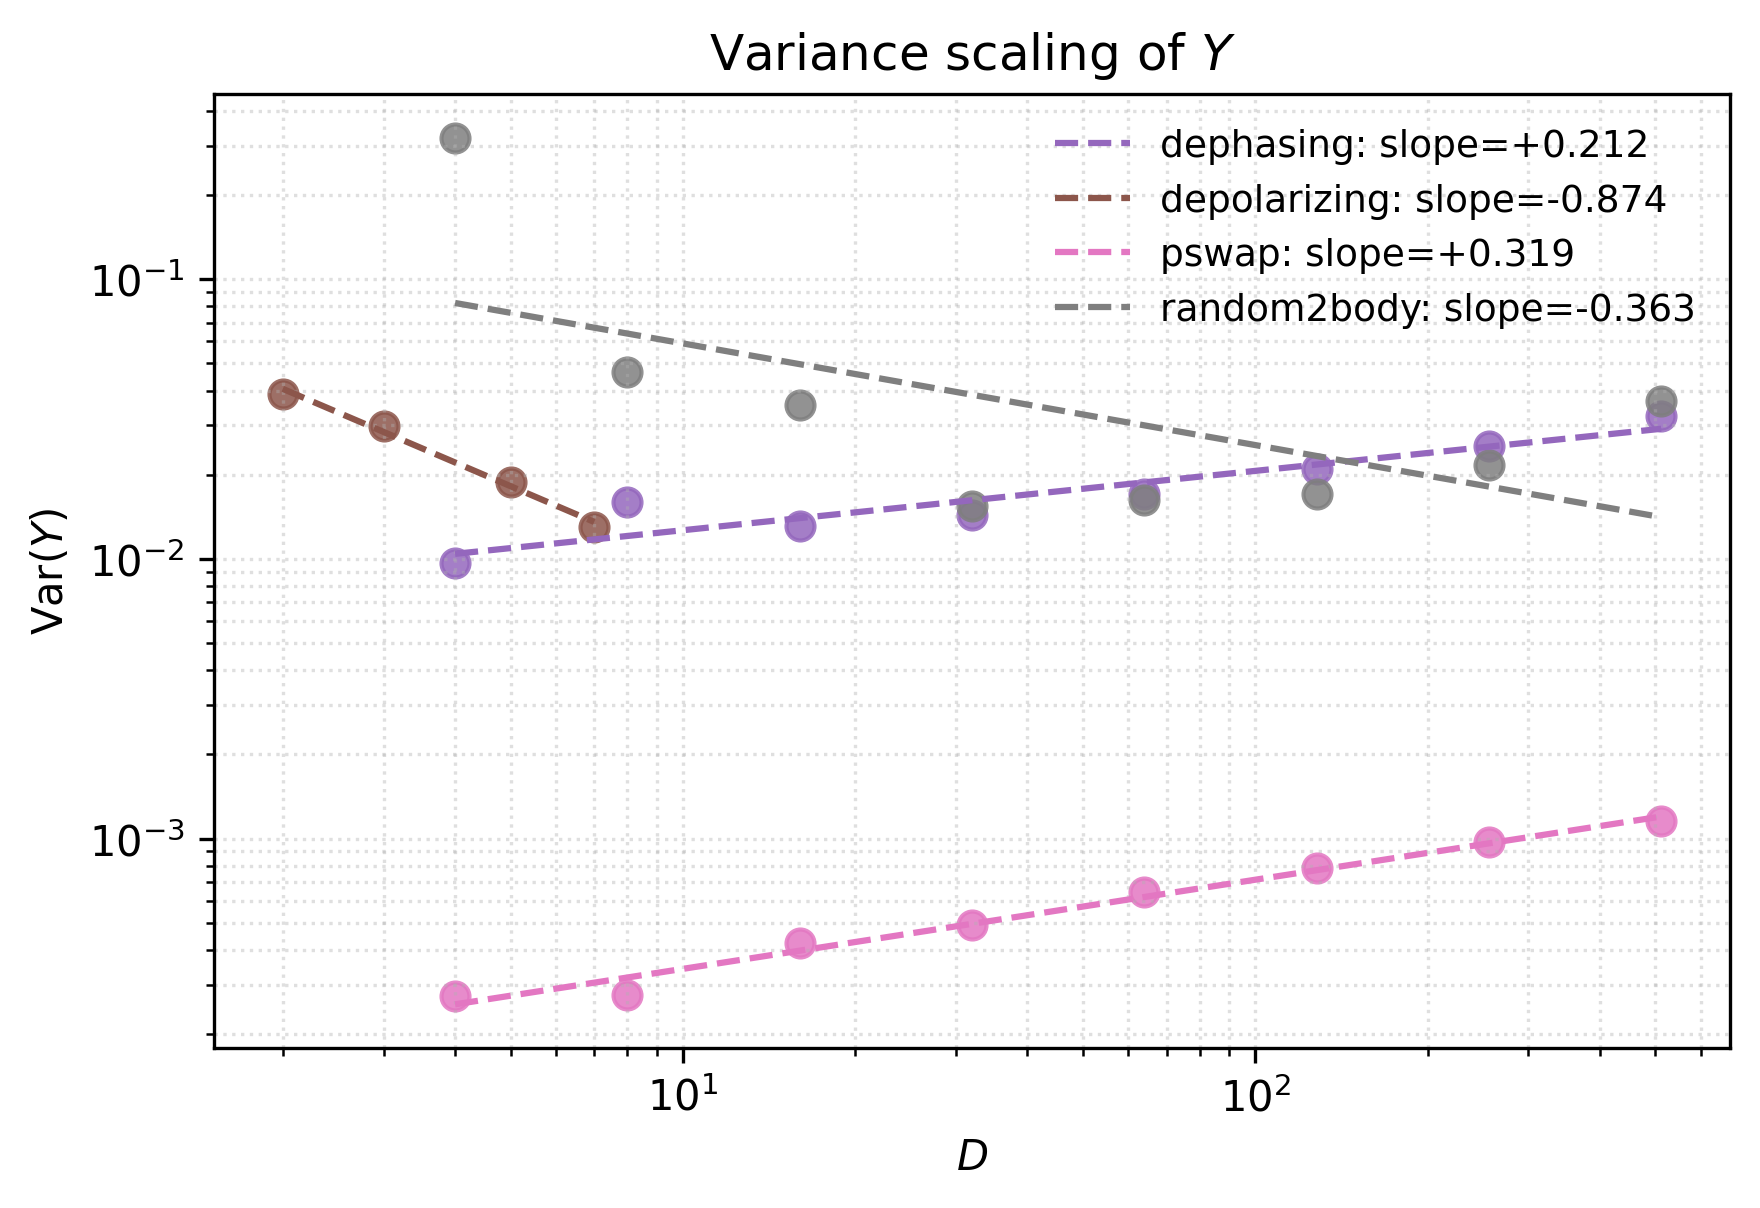
\includegraphics[width=0.7\linewidth]{../figures/phase3_varY_scaling.png}
\caption{Variance scaling $\Var(\Y)$ vs $D$.}
\end{figure}

\begin{figure}[h]
\centering
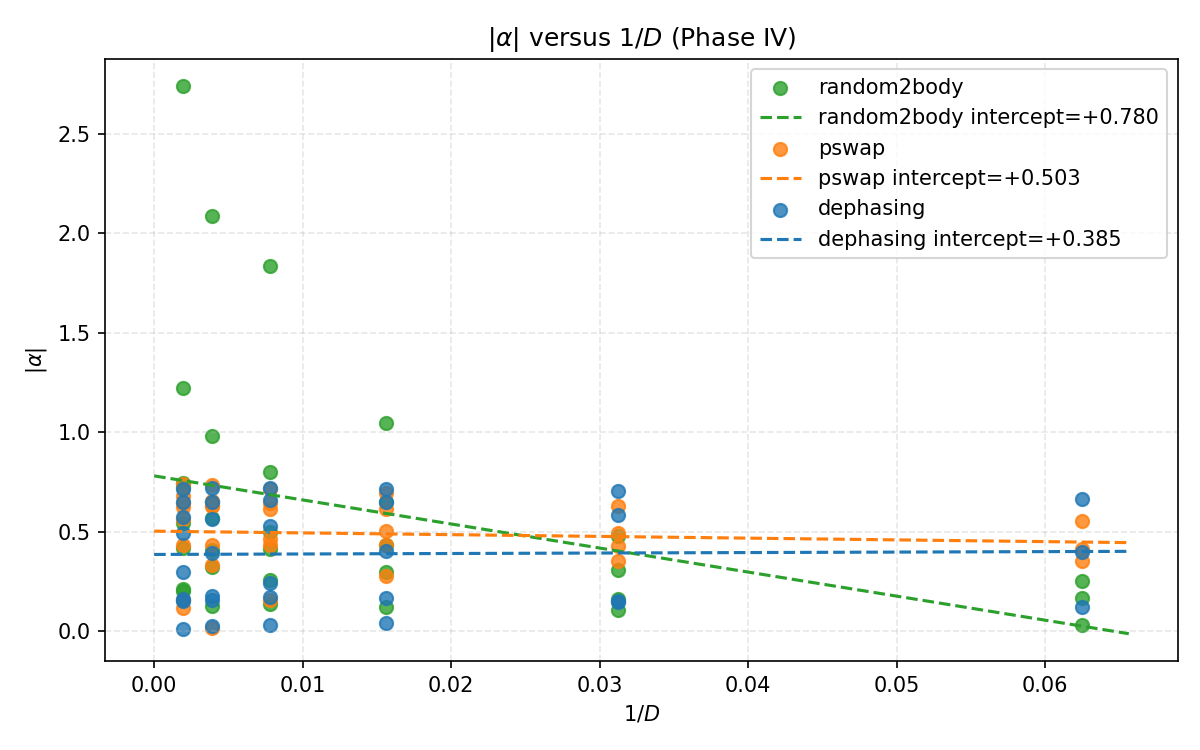
\includegraphics[width=0.7\linewidth]{../figures/phase4_alpha_vs_invD.png}
\caption{$|\alpha|$ versus $1/D$ (Phase IV).}
\label{fig:phase4-alpha-invD}
\end{figure}

\begin{figure}[h]
\centering
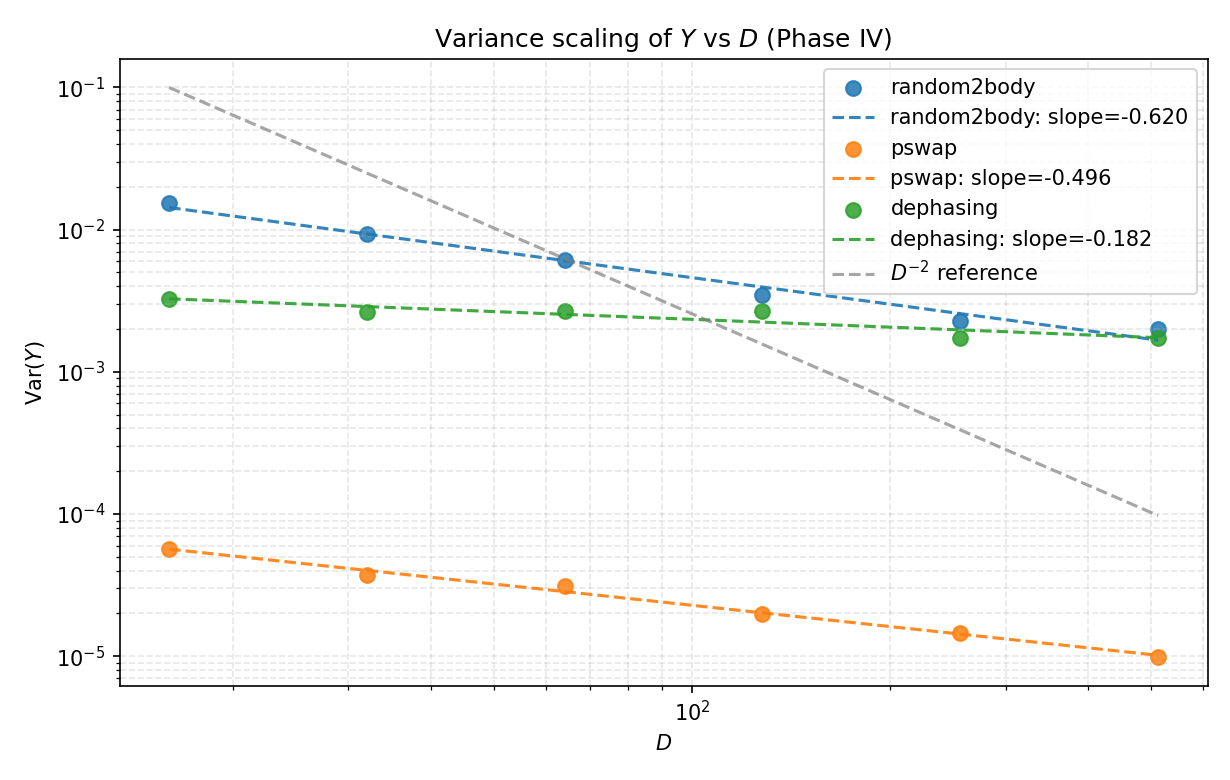
\includegraphics[width=0.7\linewidth]{../figures/phase4_varY_scaling.png}
\caption{Variance scaling $\Var(Y)$ vs $D$ (Phase IV).}
\label{fig:phase4-vary}
\end{figure}

\bibliographystyle{unsrt}
\bibliography{references}

\clearpage
\appendix
\section{Curvature--Information Concentration and Universality}\label{app:theorem}

\paragraph{Setting and notation.}
Let $S$ be a $d_S$-dimensional system and $E$ an environment with $d_E$ levels, so the joint Hilbert space has
$D = d_S d_E$.
Consider one step of an open evolution realized by a Stinespring dilation:
$\rho_S \mapsto \rho_S' = \mathrm{Tr}_E\!\left[ U\, (\rho_S \otimes |0\rangle\!\langle 0|_E )\, U^\dagger \right]$,
where $U$ is drawn from a \emph{unitary 2-design} on $U(D)$.
Define
\[
\deff(\rho_S') \equiv \frac{1}{\mathrm{Tr}[(\rho_S')^2]},\qquad
\A^2 \equiv \arccos^2\!\Big( \sqrt{F(\rho_S,\rho_S')} \Big),\qquad
\I \equiv I(S\!:\!E)_{\rho_{SE}'},
\]
and the curvature--information invariant
\[
\Y \;\equiv\; \sqrt{\deff(\rho_S') - 1}\;\frac{\A^2}{\I}.
\]
We study the log--log slope
\(
\alpha \equiv \frac{d \log \Y}{d \log( \deff - 1)}.
\)
Unless otherwise noted $d_S$ is fixed and $D \to \infty$ (i.e., $d_E \to \infty$).

\begin{theorem}[Curvature--Information Concentration and Flatness under 2-designs]
\label{thm:CI}
Let $U$ be sampled from a unitary 2-design on $U(D)$ with $D=d_S d_E$, fixed $d_S$, and $D\to\infty$.
Then there exists a constant $Y_0$ (independent of $D$, of the initial $\rho_S$, and of microscopic details) such that
\begin{align}
\mathbb{E}[\,\Y\,] &= Y_0 + O(D^{-1}),\\
\mathrm{Var}(\Y) &= \Theta(D^{-1}),\\
\mathbb{E}[\alpha] &= O(D^{-1}), \qquad \mathrm{Var}(\alpha) = \Theta(D^{-1}).
\end{align}
Consequently, the signed slope $\alpha$ converges to $0$ in mean and concentrates with typical magnitude
$|\alpha| = O_\mathbb{P}(D^{-1/2})$, and any regression of $\alpha$ against $1/D$ has intercept $b \to 0$ with
$|b| = O(D^{-1})$.
\end{theorem}

\paragraph{Interpretation.}
The mean $\Y$ stabilizes to a universal constant $Y_0$ up to $D^{-1}$ corrections, while the finite-size variance obeys
the \emph{variance law} $\Var(\Y) \sim c\,D^{-1}$ confirmed numerically in Phases~VIII--IX. Flatness means the slope of
$\log \Y$ against $\log(\deff-1)$ averages to $0$ and its fluctuations shrink like $D^{-1/2}$; thus signed-$\alpha$
confidence intervals include $0$ at large $D$ and the $\alpha$ vs $1/D$ intercept tends to $0$.

\paragraph{Proof sketch.}
Write $\rho_S' = \mathrm{Tr}_E[U(\rho_S\otimes|0\rangle\langle 0|)U^\dagger]$ and set $\delta\rho\equiv \rho_S' - \rho_S$.
Using 2-design (second-moment) Weingarten identities up to fourth order, one has the standard reduced-state concentration:
\[
\mathbb{E}[\rho_S'] = \frac{I_{d_S}}{d_S} + O(D^{-1}),\quad
\mathbb{E}[\mathrm{Tr}(\rho_S'^2)] = \frac{1}{d_S} + O(D^{-1}),\quad
\mathrm{Var}[\mathrm{Tr}(\rho_S'^2)] = \Theta(D^{-1}).
\]
Thus $\deff(\rho_S')-1$ is tight and has $D^{-1}$-scale fluctuations.
In the Bures geometry, for small perturbations $\A^2 = \tfrac14\, g_{\mathrm{Bures}}(\delta\rho,\delta\rho) + O(\|\delta\rho\|^3)$,
and isotropy of the 2-design implies $\mathbb{E}[\A^2] = c_1 D^{-1} + O(D^{-2})$ with $\mathrm{Var}(\A^2)=\Theta(D^{-1})$.
For the mutual information, with a pure global dilation one has $\I=2 S(\rho_S')$; Page-type concentration yields
$\mathbb{E}[\I] = I_0 + O(D^{-1})$ and $\mathrm{Var}(\I)=\Theta(D^{-1})$.
Applying the delta method to $\Y=\sqrt{\deff-1}\,\A^2/\I$ (a smooth function of concentrated quadratic functionals) gives
the stated rates.

\paragraph{Corollary (Universality/Structure/Twirl).}
(i) For chaotic/isotropic evolutions (random 2-body at mixing time; depolarizing/twirled channels), the
assumptions hold and Theorem~\ref{thm:CI} applies (flat $\alpha$, $D^{-1}$ variance). \\
(ii) For structured/integrable dynamics (partial-swap, dephasing, amplitude damping without twirl),
the isotropy hypothesis fails and $\alpha$ deviates from $0$; \emph{however}, \emph{unitary twirling} (pre/post conjugation by local 2-designs) restores isotropy and hence the theorem’s conclusions.

\paragraph{Finite-size scaling form.}
Under the theorem’s hypotheses,
\[
\mathbb{E}[|\alpha|^2] = \Theta(D^{-1}) \;\Rightarrow\;
\mathbb{E}[|\alpha|] = O(D^{-1/2}),\quad
\Var(\Y) = \Theta(D^{-1}),\quad
\mathbb{E}[\Y] = Y_0 + O(D^{-1}).
\]
Empirically (Phases VII–IX) weighted least squares of $\alpha$ vs $1/D$ give intercept CIs that shrink to $0$,
and $\log\Var(\Y)$ vs $\log D$ has slope $\beta \approx -1$ with tight bootstrap CIs.

\paragraph{Experimental protocol (Clifford twirl).}
\emph{System.} 2–3 qubits on a trapped-ion or superconducting platform.\\
\emph{Channel and twirl.} Implement a noisy channel on a target qubit and conjugate by random Clifford unitaries (local 2-design).\\
\emph{Measurements.} Single-qubit tomography to estimate $\rho_S$ and $\rho_S'$, compute $\A^2 = \arccos^2\!\sqrt{F(\rho_S,\rho_S')}$,
estimate $S(\rho_S')$ (hence $\I=2S(\rho_S')$), and purity for $\deff$.\\
\emph{Scaling.} Increase effective $D$ by adding idle-coupled ancillas (or by increasing mixing depth), repeat to obtain $\{(\deff,\Y)\}$ pairs.\\
\emph{Predictions.} (1) Signed $\alpha$ CI includes $0$ at each depth; (2) $\Var(\Y)$ vs $D$ has slope $\approx -1$ on log–log axes; (3) $|\alpha|$ vs $1/D$ extrapolates to intercept $0$ within CI.


\end{document}
